\chapter{Web Interface}
\label{ch:interface}
\section{Main Menu}
\label{sec:main menu}
Upon logging in, the {\imp Main Menu} will be in plain sight (as shown in~\autoref{fig:\ares Web Interface}). It displays the Current Course table. If the instructor has promised to bring a personal copy to the library, there will appear an ``Awaiting Supply by Instructor'' table. 
\vspace*{3.5ex}

\begin{figure}[h]
    \centering
    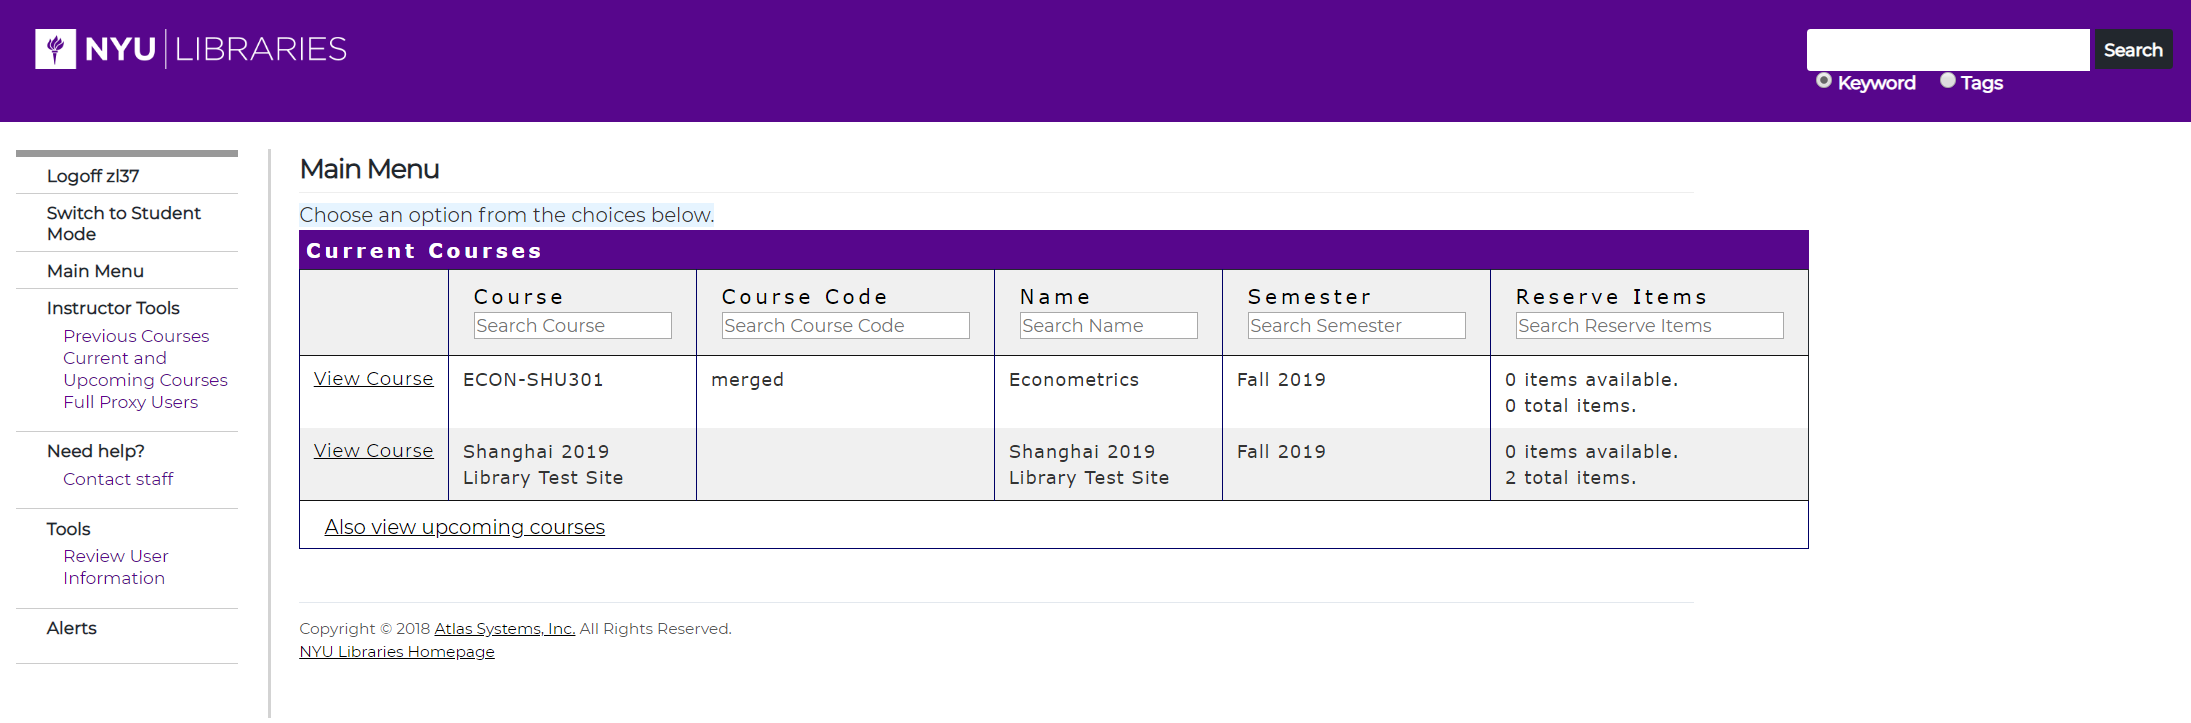
\includegraphics[width=\textwidth]{interface}
    \caption{Main Menu of \ares Web Interface}
    \label{fig:\ares Web Interface}
\end{figure}
\vspace*{2.5ex}

If you do not find the course you are expecting, try ``Also view upcoming courses'' at the table bottom. But when the course information of future semesters has not been updated in \ares system, nothing new will appear.

\section{Side Bar}
\label{side bar}


\begin{wrapfigure}{o}{0.25\textwidth}
    \centering
    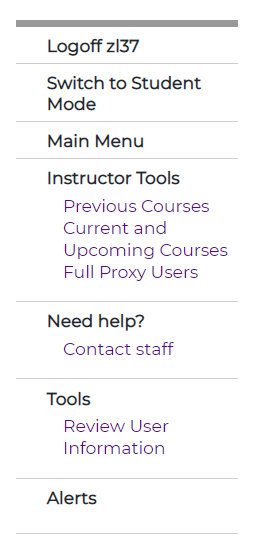
\includegraphics[width=0.25\textwidth]{sidebar}
    \caption{Side Bar}
    \label{fig: side bar}
\end{wrapfigure}

The left side bar offers some more features to explore:

Instructors can switch to Student Mode to get a feel of their interface, quite similar though. 

The {\imp Instructor Tools} provides some key functions. ``Previous Courses'' allows to view your past courses and items. ``Current and Upcoming Courses''  will display courses that belong to the current semester, as well as those of any upcoming semesters that instructors have early access to (as soon as course data is loaded in Albert). As to ``Full Proxy Users'', reference \autoref{ch:proxy} for more information.
\clearpage

\section{Course Home}
\label{sec: course page}
Click \uline{View Course} in the first column of the Current Courses table, and then you will enter the Course Home page, where \textbf{Course Details} are shown.

\vspace*{3ex}
\begin{figure}[h]
    \centering
    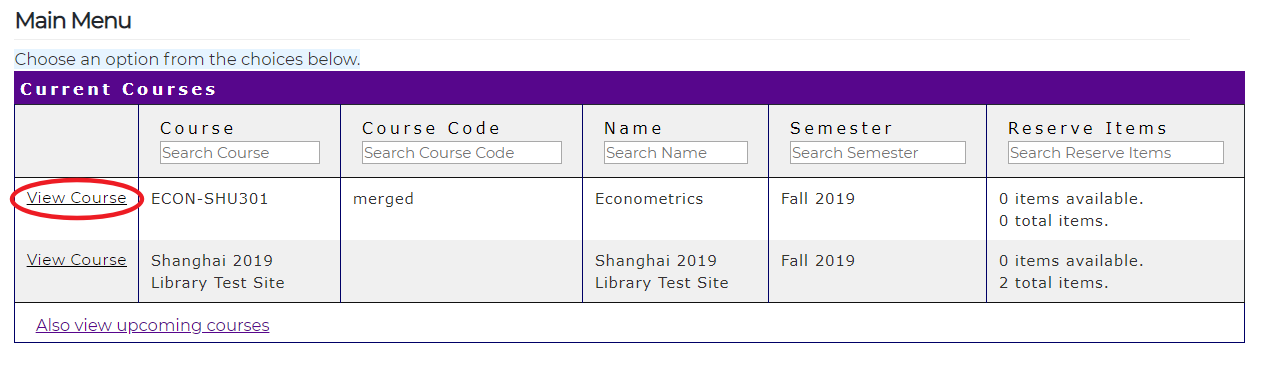
\includegraphics[width=\textwidth]{viewcourse}
    \caption{View Course}
    \label{fig:view course}
\end{figure}
\vspace*{2ex}

Once in a course, listed in the table are the {\imp Reserve Items} for this course. The \uline{Show Details} option allows you to view an item, which will be detailed in \autoref{ch:organize}, and \uline{Edit} to make changes to it.

\vspace*{3ex}
\begin{figure}[h]
    \centering
    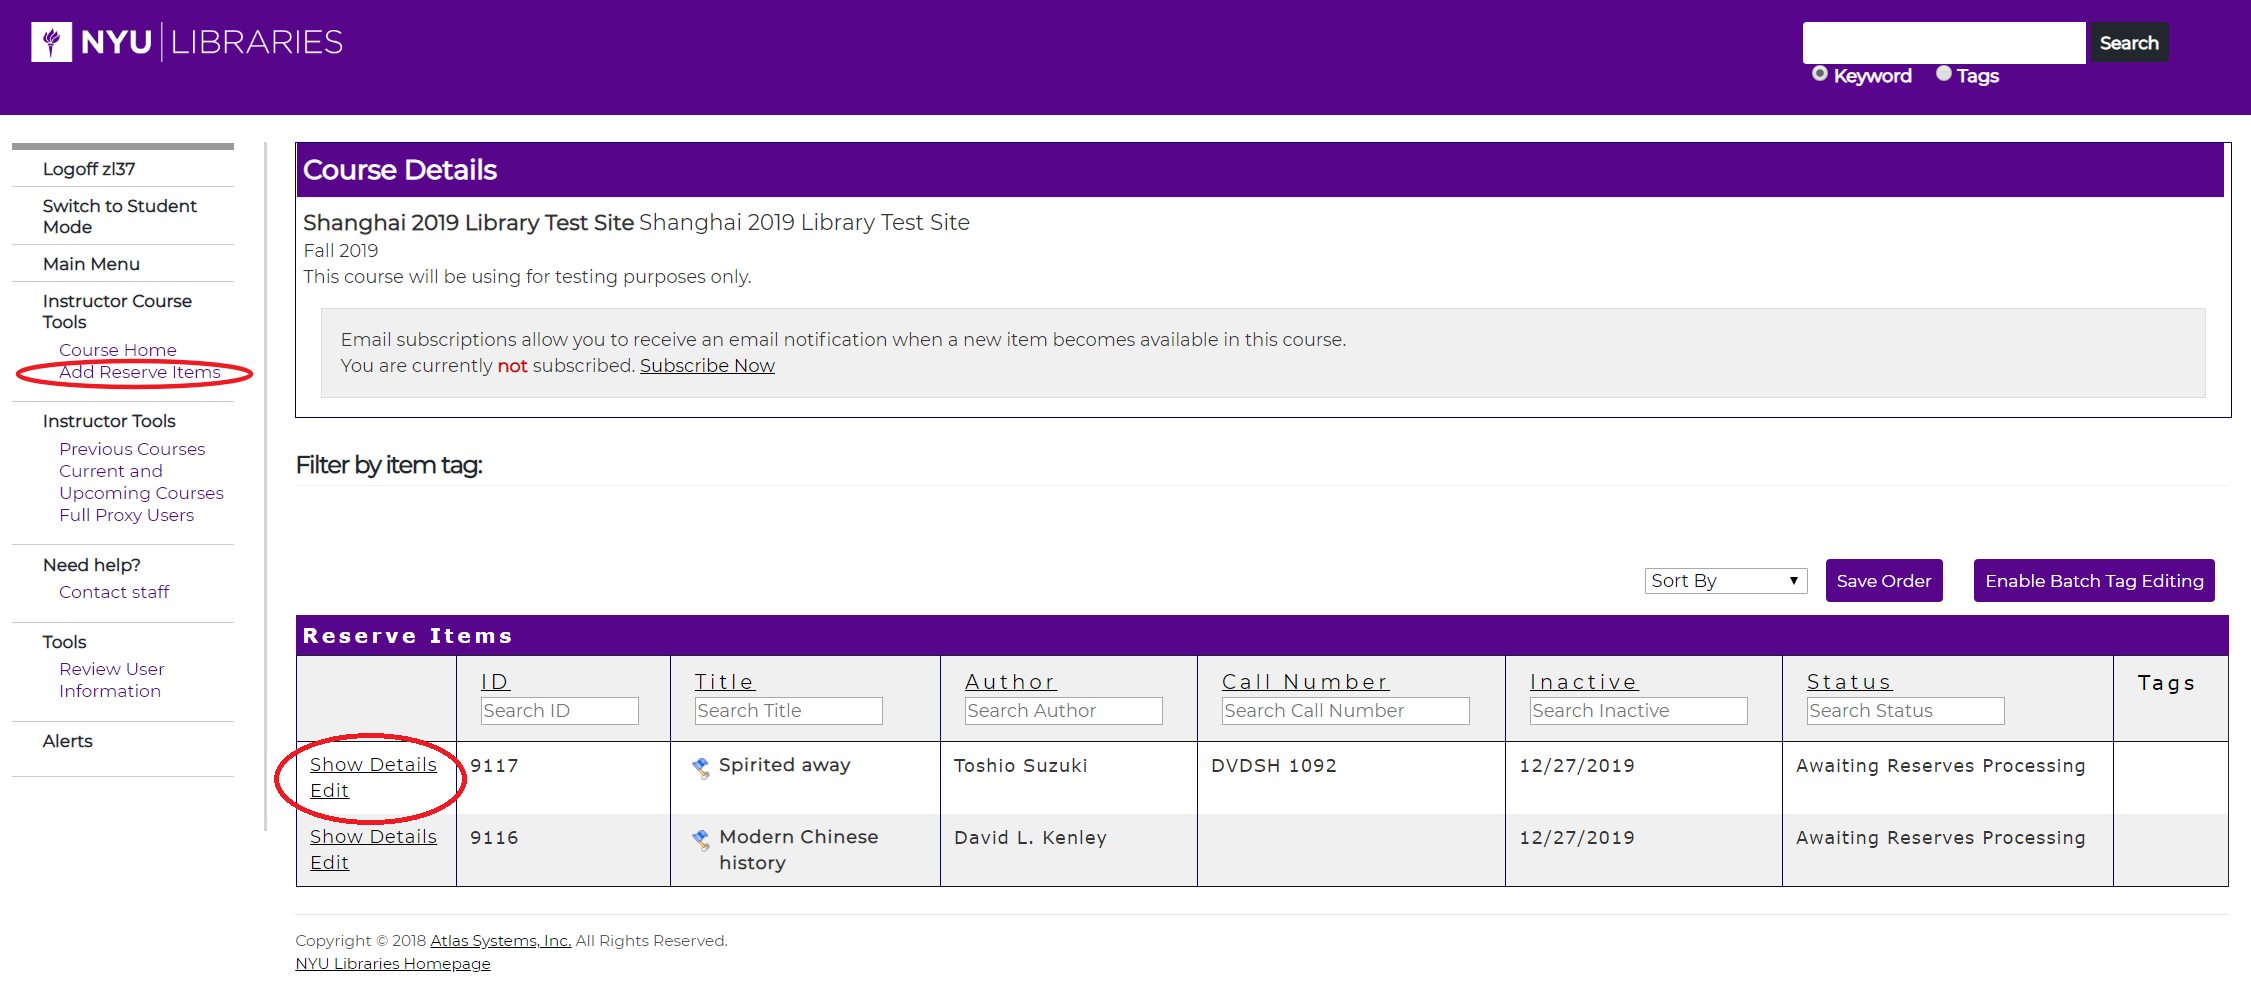
\includegraphics[width=\textwidth]{coursepage}
    \caption{Course Home}
    \label{fig:course home}
\end{figure}
\vspace*{6ex}

\begin{notebox}
    When you cannot edit an item, this means the library staff have started processing your requests and therefore the item has been locked. A notification will appear under {\imp Main Menu}: 
    \tcblower
    \areswarning{Due to staff processing, this item is currently unable to be modified.}
    \label{note: notedit}
\end{notebox}
\vspace*{3ex}


Yet before looking into a specific item, let's first move to the most important part of this Guide---{\imp Add Reserve Items}.